\documentclass{xcpc}
\usepackage{caption}
\usepackage{subcaption}
\usepackage{geometry}
\usepackage{boxedminipage}
\usepackage{makecell}
\usepackage{xcolor}
\geometry{a4paper,scale=0.8}
\usetikzlibrary{patterns}
\schoolshort{JSUT}
\schoolname{Jiangsu University of Technology}
\location{Changzhou, Jiangsu Province}
\logo{jsuttext}

\begin{document}
	\pagestyle{empty}
	
	\begin{center}
		\vspace*{12em}
		
		\begin{figure}[htbp]
			\centering
			\begin{minipage}[t]{0.48\textwidth}
				\centering
				\icpclogo{0.15}
			\end{minipage}
			\begin{minipage}[t]{0.48\textwidth}
				\centering
				\includegraphics[width=6cm]{jsuttext}
			\end{minipage}
		\end{figure}
		
		{\huge\bf 2025 \schoolshort Collegiate Programming Contest\\\schoolname\\\location}
	\end{center}
	\tableofcontents
	\clarification{Warn up contest.}
	\clearpage 
	\pagestyle{fancy}
	\begin{problem}{I will AK JSUTCPC}
		\begin{boxedminipage}[c][1cm][t]{22em} 
			Time Limit: 1 second
			
			Memory Limit: 256 megabytes
		\end{boxedminipage}
		
		Welcome to JSUTCPC!
		
		AK means All Killed, which indicates that all questions in a competition have been accepted. Timothy hopes that everyone can not only AK every competition in the future, but also AK all the troubles in life. Thank you for participating in JSUTCPC!
		
		So Timothy considers all letters A to K in the alphabetical list as lucky letters, and the question setters of various competitions after JSUTCPC will definitely not let you get AK, so you need to judge whether the letters they give are lucky letters.
		
		\begin{inputdes}
			The first line give a uppercase letter c(c is a capital letter from A to Z and not contains A and K). Indicates the letter given by the question setter.
		\end{inputdes}
		
		\begin{outputdes}
			If c is a lucky letter, then output $\tt{true}$, otherwise output $\tt{false}$.
			
			Answers are not case sensitive. For example, $\tt{True}$, $\tt{TRUE}$, $\tt{TrUe}$ and $\tt{trUE}$ can all mean that c is lucky letter.
		\end{outputdes}
		
		\section*{Example}
		
		\begin{table}[h]
			\begin{tabular}{|l|l|}
				\hline
				\textbf{Standard Input} & \textbf{Standard Output} \\ \hline
				\makecell[l]{$\tt{F}$} & \makecell[l]{$\tt{true}$} \\ \hline
				\makecell[l]{$\tt{W}$} & \makecell[l]{$\tt{false}$} \\ \hline
				\makecell[l]{$\tt{J}$} & \makecell[l]{$\tt{true}$} \\ \hline
			\end{tabular}
		\end{table}
		
		\section*{Note}
		
		For the first example, F comes after A and before K in alphabetical order, so the output is $\tt{true}$.
	\end{problem}
	
	\begin{problem}{Bracket or Brackets?}
		\begin{boxedminipage}[c][1cm][t]{22em} 
			Time Limit: 1 second
			
			Memory Limit: 256 megabytes
		\end{boxedminipage}
		
		Timothy is the old member of Network and xcpc. He speaks strangely in the QQ group. He always adds a bracket after a sentence (.
		
		As above. And Papers says that if Timothy's ending brackets are not paired when he speaks, that is:
		\begin{enumerate}
			\item An opening bracket must be closed by a closing bracket of the same type.
			\item Opening brackets must be closed in the correct order.
			\item Every close bracket has a corresponding open bracket of the same type.
		\end{enumerate}
		
		If the above three conditions are met, it means he is joking. Otherwise, it means he is making a serious statement. Please help Papers decide if Timothy is joking.
		
		\begin{inputdes}
			The first line give a string s(s.size()$\leq 10^4$) containing just the characters `(', `)', `\{', `\}', `[' and `]', determine if the input string is valid.
		\end{inputdes}
		
		\begin{outputdes}
			If Timothy is joking, output $\tt{true}$, otherwise output $\tt{false}$.
			
			Answers are not case sensitive. For example, $\tt{True}$, $\tt{TRUE}$, $\tt{TrUe}$ and $\tt{trUE}$ can all mean that Timothy is joking.
		\end{outputdes}
		
		\section*{Example}
		
		\begin{table}[h]
			\begin{tabular}{|l|l|}
				\hline
				\textbf{Standard Input} & \textbf{Standard Output} \\ \hline
				\makecell[l]{$\tt{()}$} & \makecell[l]{$\tt{true}$} \\ \hline
				\makecell[l]{$\tt{(]}$} & \makecell[l]{$\tt{false}$} \\ \hline
				\makecell[l]{$\tt{([])}$} & \makecell[l]{$\tt{true}$} \\ \hline
			\end{tabular}
		\end{table}
		
	\end{problem}
	
	\begin{problem}{Trapping Rain Water}
		\begin{boxedminipage}[c][1cm][t]{22em} 
			Time Limit: 5 seconds
			
			Memory Limit: 256 megabytes
		\end{boxedminipage}
		
		Given $n$ non-negative integers representing an elevation map where the width of each pillar is 1, compute how much water it can trap after raining.
		
		\begin{inputdes}
			The first line is an integer $n$, which represents the number of pillars.
			
			The second line contains $n$ integers representing the heights of the pillars.
		\end{inputdes}
		
		\begin{outputdes}
			An integer representing the number of units that can catch rainwater.
		\end{outputdes}

		\section*{Example}
		
		\begin{table}[h]
			\begin{tabular}{|l|l|}
				\hline
				\textbf{Standard Input} & \textbf{Standard Output} \\ \hline
				\makecell[l]{$\tt{12}$\\$\tt{0\ 1\ 0\ 2\ 1\ 0\ 1\ 3\ 2\ 1\ 2\ 1}$} & \makecell[l]{$\tt{6}$} \\ \hline
				\makecell[l]{$\tt{6}$\\$\tt{4\ 2\ 0\ 3\ 2\ 5}$} & \makecell[l]{$\tt{9}$} \\ \hline
			\end{tabular}
		\end{table}
		
		\section*{Note}
		
		For the first example, as shown in the figure, the shaded area is the water volume of 6.
		
		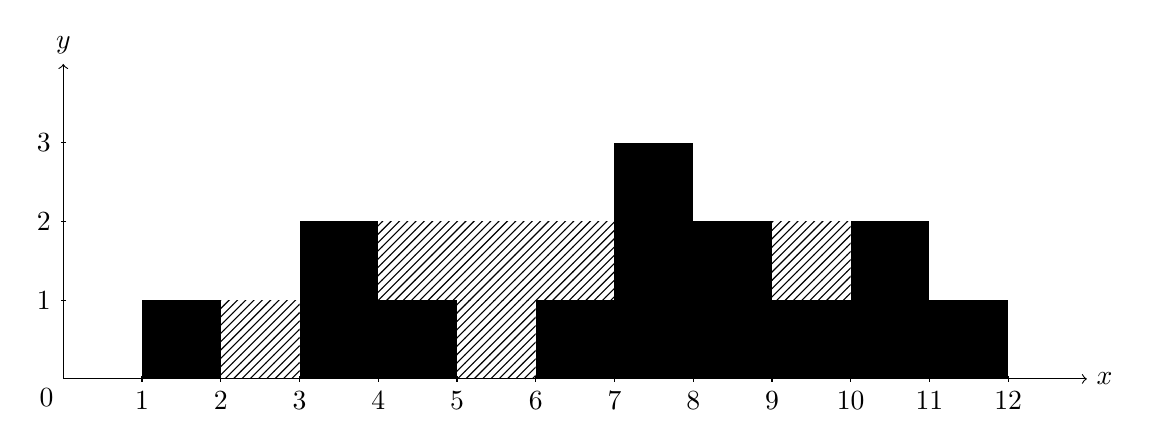
\begin{tikzpicture}
			% 绘制X轴
			\draw[->] (0,0) -- (13,0) node[right] {$x$};
			% 绘制Y轴
			\draw[->] (0,0) -- (0,4) node[above] {$y$};
			% 标注坐标原点
			\node[below left] at (0,0) {0};
			% 标注X轴刻度
			\foreach \x in {1,2,3,4,...,12}
			\draw (\x,1pt) -- (\x,-1pt) node[anchor=north] {\x};
			% 标注Y轴刻度
			\foreach \y in {1,2,3}
			\draw (1pt,\y) -- (-1pt,\y) node[anchor=east] {\y};
			
			\fill (1,0) rectangle (2,1);
			\fill (3,0) rectangle (4,2);
			\fill (4,0) rectangle (5,1);
			\fill (6,0) rectangle (7,1);
			\fill (7,0) rectangle (8,3);
			\fill (8,0) rectangle (9,2);
			\fill (9,0) rectangle (10,1);
			\fill (10,0) rectangle (11,2);
			\fill (11,0) rectangle (12,1);
			
			\fill[pattern=north east lines] (2,0) rectangle (3,1);
			\fill[pattern=north east lines] (4,1) rectangle (7,2);
			\fill[pattern=north east lines] (5,0) rectangle (6,1);
			\fill[pattern=north east lines] (9,1) rectangle (10,2);
		\end{tikzpicture}
	\end{problem}
	
	\begin{problem}{Fishing}
		\begin{boxedminipage}[c][1cm][t]{22em} 
			Time Limit: 1 second
			
			Memory Limit: 512 megabytes
		\end{boxedminipage}
		
		Timothy and his friends went fishing on the island. They looked at the map before leaving.
		
		This area is $m \times n$ and can be viewed as a two-dimensional array, where the integer $t_{ij}>0$ at the subscript $(i, j)$ indicates that this area is water and has $t_{ij}$ fish, and if $t_{ij}=0$, it means that this is land.
		
		Timothy can start from any water grid $t_{ij}>0$ and perform the following operations any number of times。 Catch all the fish at grid $(i, j)$, or move to an adjacent water grid.
		
		What is the maximum number of fish Timothy can catch?
	
	
	\begin{inputdes}
		The first line contains two integers $m,n$ representing the region of $m\times n$.
		
		The next $m$ rows, each with $n$ numbers, represent the map information of the water area in this piece, where the $i$th row and $j$th column represent $t_{ij}$. The numbers are separated by spaces.
	\end{inputdes}
	
	\begin{outputdes}
		Please output the maximum number of fish that can be caught under Timothy's optimal strategy. If there is no water grid, please output 0.
	\end{outputdes}
	
	\section*{Example}
	
	\begin{table}[h]
		\begin{tabular}{|l|l|}
			\hline
			\textbf{Standard Input} & \textbf{Standard Output} \\ \hline
			\makecell[l]{$\tt{4\ 4}$\\$\tt{0\ 2\ 1\ 0}$\\$\tt{4\ 0\ 0\ 4}$\\$\tt{1\ 0\ 0\ 4}$\\$\tt{0\ 3\ 2\ 0}$} & \makecell[l]{$\tt{7}$} \\ \hline
			\makecell[l]{$\tt{1 3}$\\$\tt{1\ 3\ 9}$} & \makecell[l]{$\tt{13}$} \\ \hline
		\end{tabular}
	\end{table}
	
	\section*{Note}
	
	For the first example, Timothy can start at square (1,3), catch 3 fish, then move to square (2,3) and catch 4 fish.
	\end{problem}
\end{document}